\chapter{Compilation and Linking}
The process that bridges the source code to machine code and the final executable is the compilation; human readable
code is translated into binary instructions that can be read and executed by the CPU. The compilation of C code for
instance requires 4 steps:
\begin{enumerate}
    \item Preprocessing;
    \item Compilation;
    \item Assembly;
    \item Linking.
\end{enumerate}
Most of the times these phases are merged into a single one by modern compilers but in reality they are carried out
separately.
\begin{figure}[!htbp]
    \centering
    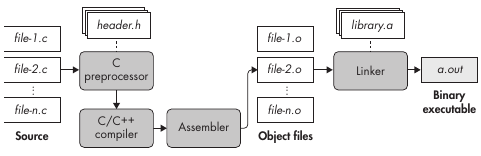
\includegraphics[scale=0.7]{./pics/compilation.png}
    \caption{Compilation phases}
    \label{comp}
\end{figure}

\section{Preprocessing}
The source files to be compiled normally contains a certain number of macros (denoted by the {\ttfamily \#define})
keyword and {\ttfamily \#include} directives; in the preprocessing phase these are expanded (i.e. macros and header
files are translated into equivalent C source code). At this stage all of the headers have been "copied" into our
source code ands ready to be compiled. In gcc the output of the preprocessing step can be obtained by issuing the
command {\ttfamily gcc -E -P}.

\section{Compilation}
The compilation phase translates the processed source code into assembly language. At this stage it is possible to
invoke compiler optimisation on our code (for gcc, clang and most of the UNIX toolchain the optimisation options
range in {\ttfamily -O0-3}). Compiling directly into machine code would be too much of a daunting, if not plain
risky, task; thus it is better to have a single dedicated assembler that can handle the final translation into
machine code. The output of the compilation phase is indeed pretty much human readable with intact symbolic
information (unlike stripped binaries). In order to tell the compiler to stop at this stage we can issue the {\ttfamily
-S masm=intel} options to obtain the assembly file (*.s).

\section{Assembly}
In the assembly phase the *.s files are eventually translated into object files (with extension *.o and sometimes called
modules). The instruction here contained are in principle executable by the CPU, but there needs to be still some work
to do before having a ready-to-run executable file. Typically a single source file corresponds to a single object file.
The option to stop the full compilaòtion process at the current stage is {\ttfamily gcc -c}. The produced file conforms
to the ELF specifications and is \textbf{relocatable}; thus the file does not rely on being placed at a specific address
in memory, but they can be mapped anywhere without breaking the code logic. The term relocatable indicates that we are
dealing with an object file and not an executable. This is particularly important because normally object files are
compiled independently from each other and the assembler does not have an idea where the other object files must be
placed when assembling one; in this way they can be linked together to form the final executable.

\section{Linking}
This is the final phase of the compilation process; object files are finally linked together into a single binary
executable. In modern systems the linking phase incorporates also the LTO (Link-Time Optimisation). The \textit{linker}
(also known as \textit{link editor}) is normally a different program from the compiler. The position in memory of the
different object files is yet to be known at the current stage; furthermore each object file might be referencing data,
functions or variables contained in other object files. The address of the referenced code and data is not known and
therefore the onject files onnly contain relocation symbols that specify how the function and variable references shall
be resolved. When an object file auto-references variables and functions, the references will also be symbolic. The
arrangement of all of the modules/object files is now known and most of the symbolic references depending on the type of
library being dealt with.
There are two types of libraries:
\begin{enumerate}
    \item Static Libraries, normally identified by the *.a exrension, are merged into the binary executable so that
        every reference can be resolved at compile time;
    \item Dynamic Libraries, also called shared, are loaded into memory only once and shared among all of the binaries
        that need to use them. So instead of copying the library into every single binary these are loaded in memory
        only once.
\end{enumerate}
\subsection{Lazy Binding: how symbolic references are resolved}
When a binary is loaded into memory the dynamic linker perform last minute relocations - e.g. resolving references to
functions located in dynamically linked libraries which address is not known at compile time - when functions are
actually invoked and avoiding useless relocations unless needed (this option can be overridden with the environment
variable {\ttfamily LD\_BIND\_NOW} set to 1 when real time performance is needed).
Linking with the {\ttfamily ld -z} option has the same effect of using {\ttfamily LD\_BIND\_NOW=1}, but giving this
instruction at compile time will cause the program to use the {\ttfamily .plt.got} with 8 bytes entries as opposed to
the conventional {\ttfamily .plt} (16 bytes entries) and place all of the GOT entries into the read only {\ttfamily
.got} section.
Lazy binding is done by means of the PLT ({\ttfamily .plt} section) and the GOT ({\ttfamily .got} and {\ttfamily
.got.plt} sections); this avoids wasting time on needless relocations unless they are needed. The PLT contains executable
instructions and is indeed part of the {\ttfamily .text} segment while the {\ttfamily .got}/{\ttfamily .got.plt} are
data sections. The instructions contained in the {\ttfamily .plt} are stubs dedicated to the redirection of the call to
correct library function. The format of the PLT is as follows:
\begin{enumerate}
    \item Default Stub (the resolver);
    \item Function Stubs;
\end{enumerate}
When calling a library function in reality the program is calling the stub of the function; the procedure for the
dynamic resolution of library functions happens in 5 steps:
\begin{enumerate}
    \item The function stub begins with an indirect jump to an address in the {\ttfamily .got.plt};
    \item \label{stubid} Before the lazy binding this address in the GOT is just the address of the instruction
        immediately  following the jump, which pushes an integer onto the stack. This integer is just an identifier for
        the PLT stub in question;
    \item The following instruction jumps to the default stub which is shared among all of the PLT stubs. The default
        stub pushes the identifier, taken from the GOT, of the executable itself;
    \item The linker pushes the address fo the library function into the GOT at the corresponding entry (identified at
        step \ref{stubid});
    \item At the next function call the stub will induce the control flow to the updated GOT entry and no additional
        steps will be required.
\end{enumerate}
In other words the dynamic linker figures out the address resolution on behalf of the executable loaded into the process
by means of the PLT stubs; the linker looks up for the address at which the external symbols are located and plugs that
into the GOT so that it now points to their actual address instead of the PLT default stub (the resolver). Any
subsequent call will already have the correct address of the called function.
The role of the GOT is of paramount importance; resolving the function call by simply plugging its address into the PLT
is unsuitable for two main reasons:
\begin{itemize}
    \item It would require the {\ttfamily .text} and {\ttfamily .plt} to be writable and that would be too easy an
        attack for a melicious agent. The extra layer of indirection avoids the creation of writable code sections;
    \item Modern systems save physical memory by sharing library code among all processes. This happens because
        libraries gets loaded only once, but they are mapped to a different virtual addresses for each process. Patching
        the address into the code section would work for a single process but would break the others.
\end{itemize}

